\section{Implementation}\label{sec:impl}


We implemented the formal transformation rule for the distributed training
as a software. We designed the software to be a standalone software, so 
the ML developers can utilize the software regardless of their environment. 
The software is written in Scala; the source code and released software
is available at https://github.com/kaist-plrg/python-analyzer. 

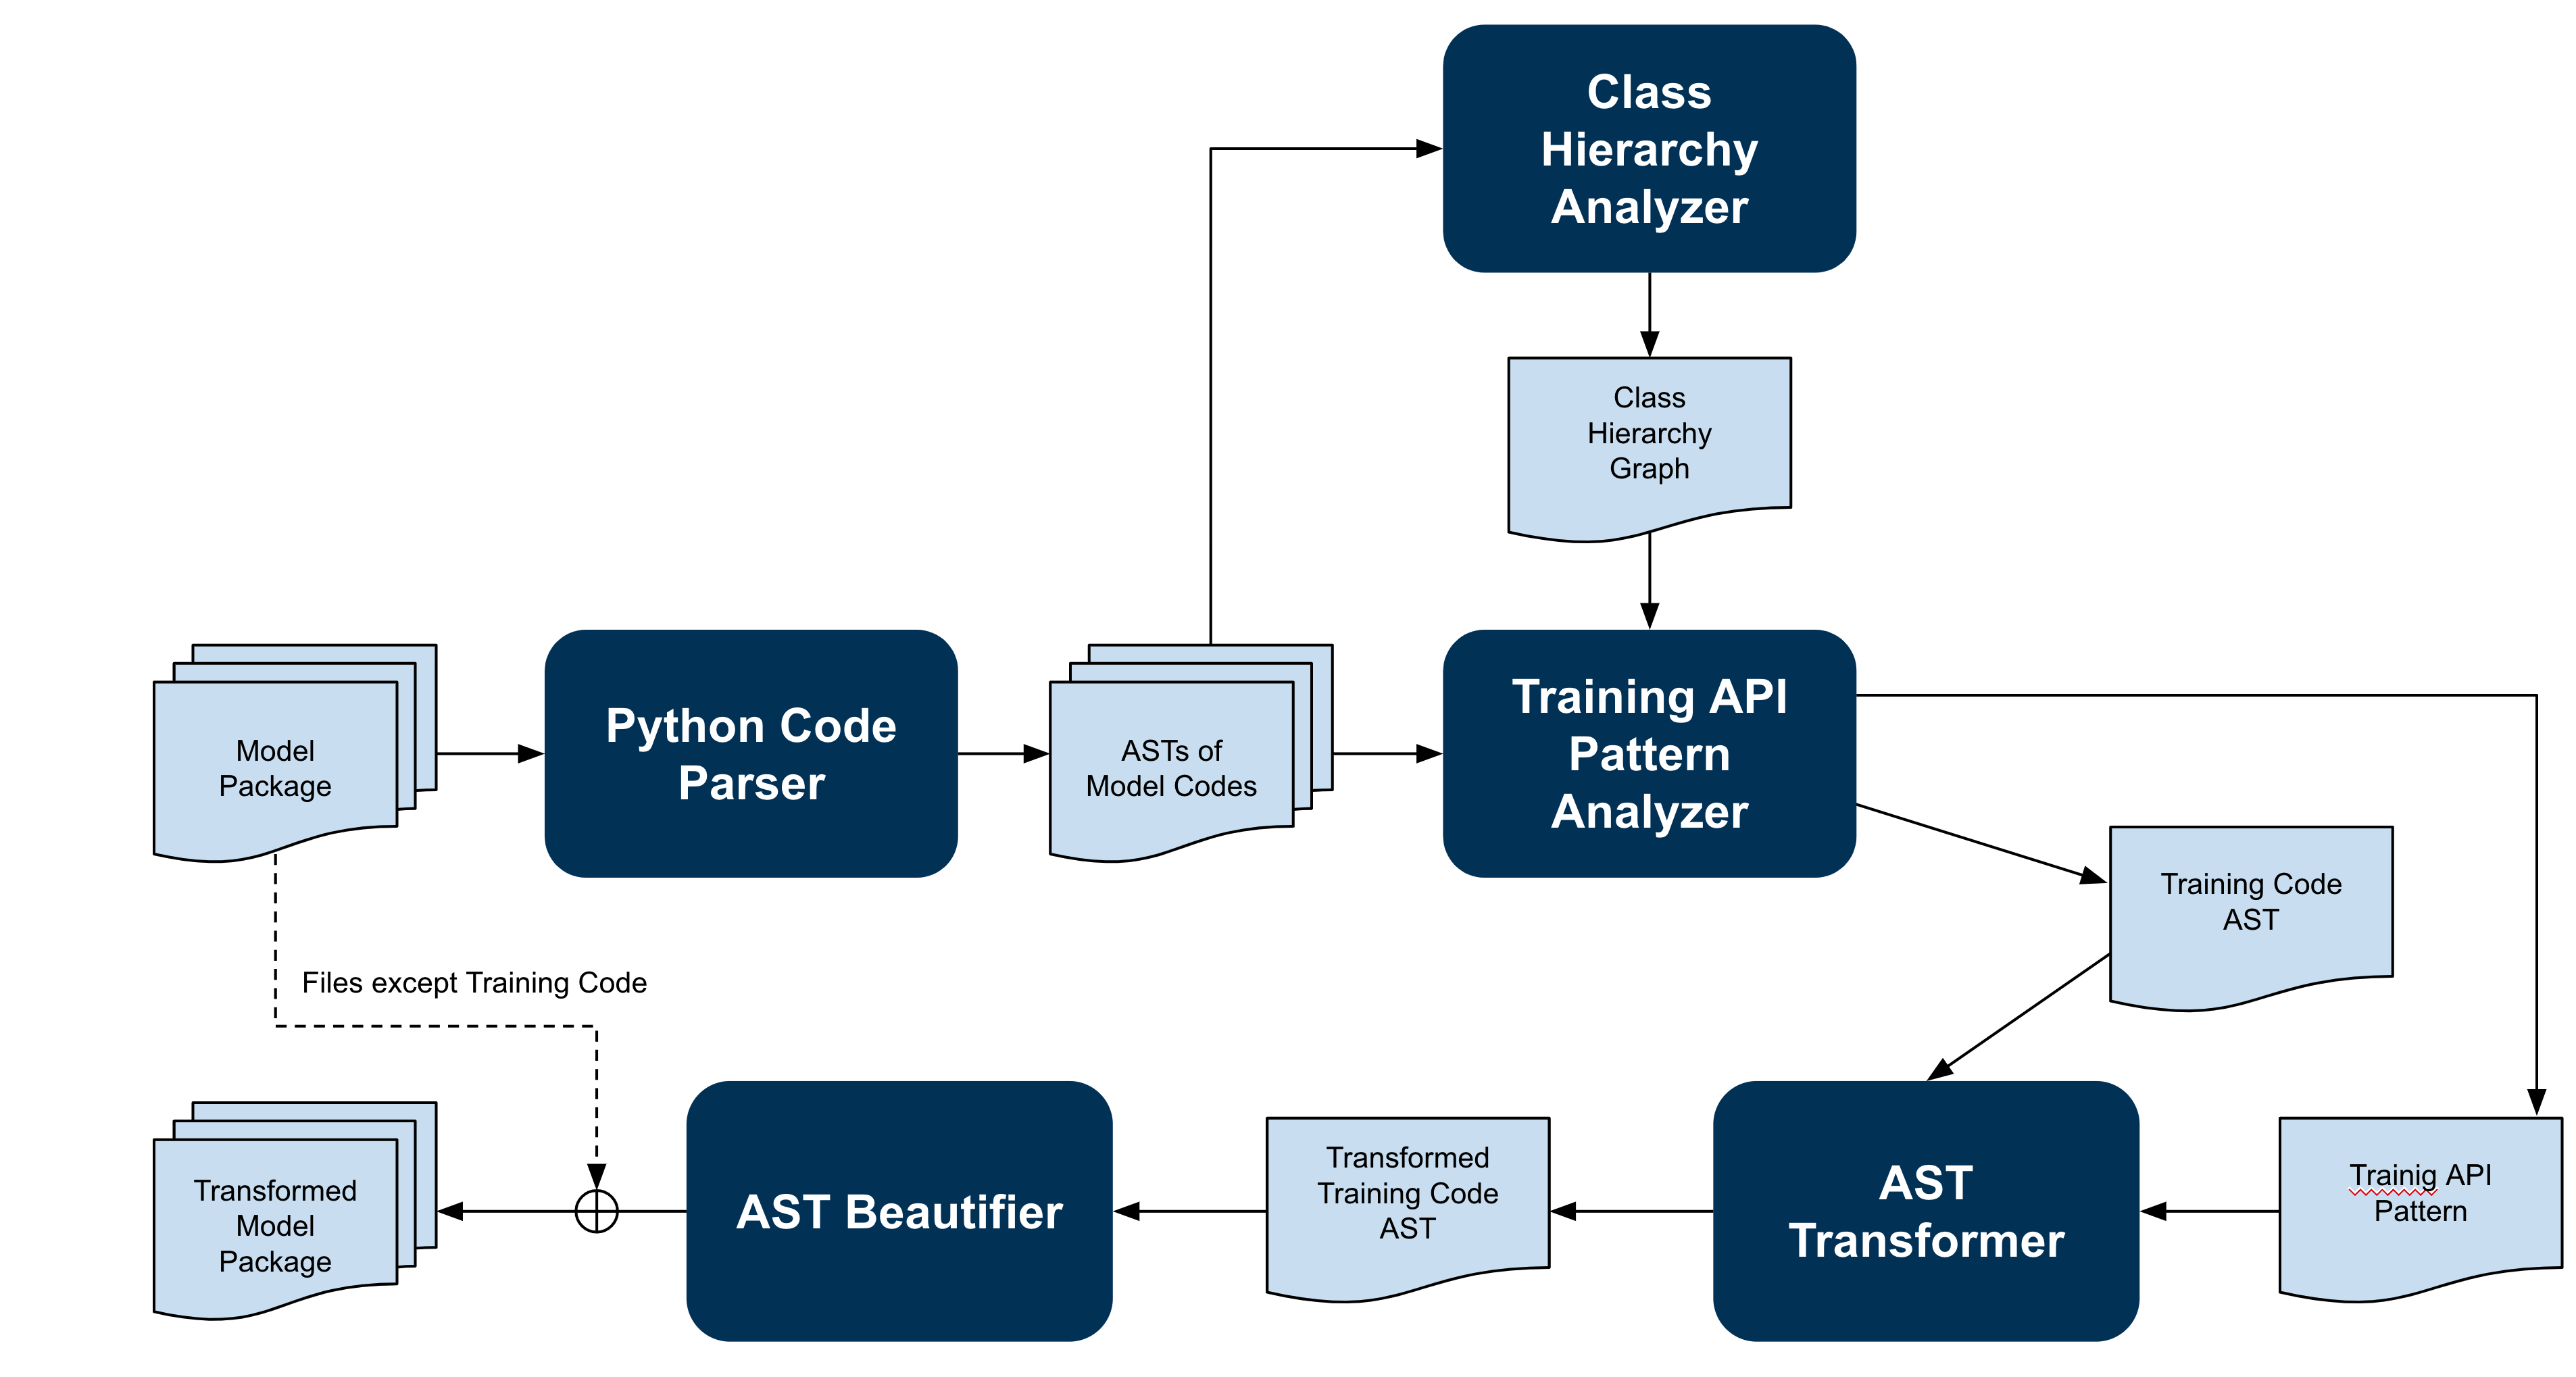
\includegraphics[width=15cm]{system_arch}

The figure illustrates the software architecture and workflow.
The software is composed of 5 modules:
Python code parser, class hierarchy analyzer,
training API pattern anlayzer, AST transformer, and AST beautifier.
The parser module parses Python codes in the input model package into 
a set of ASTs. Then the class hierarchy analyzer module 
produces a class hierarchy graph of the model package.
The training API pattern analyzer module receives the AST set and
the class hierarchy graph, identified the training code AST and
its tranining API pattern. The AST transformer module
transforms the tranining code AST according to the transformation rule.
The transformed traning code AST is printed as a Python code in the
AST beautifier module, to be merged with the original model package
and become the transformed model package.

\subsection{Class Hierarchy Analyzer}

In TensorFlow model codes, \textit{user-defined classes} inherit
training-related classes to reuse pre-defined methods.
The {\tt keras.layers.Layer} and {\tt keras.models.Model} classes 
are typical examples of the case.
Subclasses of the {\tt keras.layers.Layer} can override
the {\tt call} method to define the forward propagating computation
and automatically support gradient updates.
Subclasses of the {\tt keras.models.Model} can override
the {\tt call} method to define the model blocks
and automatically support training-related methods
such as {\tt fit} or {\tt save}. 

\lstinputlisting[language=Python]{subclass_ex.py}

The figure illustrates an example of a training code with
user-defined class inheriting {\tt keras.mopdels.Model}.
which inherits the class `tf.keras.models.Model'.
The line 4 defines a new class {\tt ResNet} that inherits the  
{\tt Layer} class. The instance of {\tt ResNet}, {\tt model}
is created at line 11. Although the class does not define
the method {\tt fit}, line 14 trains the model instance by
{\tt model.fit}. The inherited model {\tt fit}
automatically repeats the gradient descent with
given model computation and training data. 

To correctly transform training codes using user-defined classes,
the subclass relationship between user-defined classes
and TensorFlow classes should be known before training pattern analysis. 
In the above figure, for instance, the fact that the {\tt ResNet} class
is subclass of the {keras.models.Model} is essential to identify
that the code uses Keras training APIs. 
Otherwise the function call {\tt model.fit} in line 14 would
recognized as a plain function call not related to the training pattern.

The class hierarchy analyzer(CHA) module analyzes the
class subclass relationship between the 
user-defined classes and TensorFlow classes.
The module returns a class hierarchy graph(CHG) as an output.
A CHG is a directed graph structure that represents the class hierarchy.
Each node in the graph represents a class,
and each directed eadge represents a class inheritance,
where the start node indicates the child class
and the end node indicates the parent class.
Suppose the node A corresponds to the class A and node B corresponds to
the class B.
If there is a (directed) path from the node A to the node B in CHG,
then the class A is a subclass of the class B.

The CHA module gets a model code package as an input,
and creates the model package CHG as an output.
The analysis iterates over the files in the package,
and extract every subclass information available in each file.
New Python classes are defined with the {\tt class} statements.
In {\tt class} statements, newly defined class can
inherit another class by specifing the class expression
in the argument position.
The analyzer finds all {\tt class} statements from the module AST,
add the CHG node for the new class. The analyzer also adds an edge
to the parent class node if the {\tt class} statement specifies an inheritance.

After CHGs for all model code files are generated, 
they are merged into one CHG.
One caveat in the process is correct translation of class names
of submodules in the package.
The Python packaging system is closely related with the file system.
A package is specified by a directory; 
the directory name is the package name, 
and Python code files in the directory is the modules included in the package.
A package can include subpackages, which is specified
by the subdirectories, and modules in the subpackages are called submodules.
A module can access to a module in the subpackage by a qualified name,
which prefixes describe subpackage path to the target module.
This means that a same class should be specified by different qualified
names in perspectives of different subpackages.
The analyzer should also take account of the qualified names
in merging CHGs of the submodules. 
When a node in the submodule CHG is merged into the parent module CHG,
the class qualified name of the node should be prefixed with the
submodule name.
We implemented the CHG merging algorithm that constructs a correct
qualified name, and utilized it when the CHA produces the CHG for
a Python package. 

The CHA module produces a CHG for the model package and deliever to
other modules. Given the CHG, a module can compute whether a class is
subclass of another by finding path in the graph.
We implemented the CHG as a class and path-finding algorithm as
a method for the class. The path-finding algorithm is based on
a recursive depth-first search.

\subsection{Training API Pattern Analyzer}

TensorFlow provides multiple methods to define the training process.
TensorFlow 1 provides {\tt Session} API to invoke any computation
on the computation graph, and provide {\tt MonitoredTrainingSession} API to
define automatic training in terms of hooks. 
TensorFlow 2 provides {\tt GradientTape} API to define a low-level
training step, and provide {\tt Model} API to train a model without
definine low-level details.
These APIs are directly related to the training process, apart from the
model definition.
We call these APIs as \textit{training APIs}.
The model training codes are written using one of the training APIs.
To correctly transform any training codes,
the transformation software should be able to recognize the training APIs
used in the target training code and apply appropriate transformation.

We first define training API categories for TensorFlow training codes. 
We inspected open-source TensorFlow training codes to find
common pattern in their training API usage. 
As a result, we categoriezed the training codes into total four categories,
two for TensorFlow 1 and two for TensorFlow 2.




-----------

(necessity of TAPA)

As mentioned in Section 2.1, user can choose which APIs to use
when building model using TensorFlow library.
However, different transformation rule should be applied
to different usage pattern of training API.
To apply appropriate rule to each model,
the training API pattern is analyzed before the transformation.

(categories of TAP)

First, we categorized the training API pattern into 4 categories:
Session/MonitoredSession, low-level API using TensorFlow1;
Estimator, high-level API using TensorFlow1;
DistributedGradientTape, low-level API using TensorFlow2;
and Keras, high-level API using TensorFlow2.
(TODO: show the category into a table)

(how TAPA work)

Each category has unique pattern of using training API.
For example, Keras pattern is 1) making instance of model and
2) call compile and fit method of that model.
Conversly, if call expressions of the method model.compile and model.fit are detected
where model is an instance of subclass of Model class in TensorFlow library,
we categorize it as Keras pattern.

(result of TAPA)

By using training API pattern analyzer, we can figure out the API pattern.
However, it is possible that model uses more than one categories of API pattern
such as using both low-level and high-level APIs.
In this case, we reject to transform because we assumes
that each model uses only one training API pattern in the transformation rule.

\subsection{AST Transformer}
Describe detailed explanation of AST Transformer.

In transformation, it takes results of class hierarchy analysis
and training API pattern analysis, and it transforms the code
according to the rule mentioned in Section 3.2.
Because of dynamic behaviors of Python, we give up soundness
to get more complete result.
We leaves warning log with some suggestions
when transformation rule is potentially inaccurate.

